\documentclass[slovene,11pt,a4paper]{article}
%\usepackage{fullpage}
\usepackage[margin=2cm]{geometry}

\usepackage[T1]{fontenc}



%dodatni paketki:
\usepackage{braket} %paket za bra in ket
\usepackage{graphicx}
\usepackage{amsmath,amsfonts,amsthm} %matematicni paket
\usepackage{color} % omogoča barvno pisanje
\usepackage[utf8]
{inputenc}
\usepackage[slovene]{babel} % slovenski jezik/hyphenation
\usepackage{hyperref} %naredi vse povezave rečerenc, kazala,...
\numberwithin{equation}{section} % Number equations within sections (i.e. 1.1, 1.2, 2.1, 2.2 instead of 1, 2, 3, 4)
\numberwithin{figure}{section} % Number figures within sections (i.e. 1.1, 1.2, 2.1, 2.2 instead of 1, 2, 3, 4)
\numberwithin{table}{section} % Number tables within sections (i.e. 1.1, 1.2, 2.1, 2.2 instead of 1, 2, 3, 4)
\usepackage{eurosym} %za znak €

\usepackage{mathrsfs}
\usepackage{mathabx} % za kemisjke smeri in naslednje 3 vstrice
\catcode`_=12
\begingroup\lccode`~=`_\lowercase{\endgroup\let~\sb}
\mathcode`_="8000


\usepackage[margin=2cm]{geometry}



\begin{document}
\begin{titlepage}

\newcommand{\HRule}{\rule{\linewidth}{0.5mm}} % Defines a new command for the horizontal lines, change thickness here

\center % Center everything on the page

%----------------------------------------------------------------------------------------
%	LOGO
%----------------------------------------------------------------------------------------

%\includegraphics{Logo}\\[1cm] % Include a department/university logo - this will require the graphicx package
 
%----------------------------------------------------------------------------------------

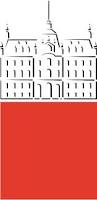
\includegraphics[width=2cm]{slike/aaa}\\[0.5cm]
 
%----------------------------------------------------------------------------------------
%	NASLOV DELA
%----------------------------------------------------------------------------------------
\textit{Univerza v Ljubljani}\\
\textit{Fakulteta za {\color{red}matematiko in fiziko}}\\[0.5cm]

\emph{Oddelek za fiziko}\\[0.5cm] % Oddelek za fiziko


%----------------------------------------------------------------------------------------
%	TITLE SECTION
%--------------------------------------------------------------------------------------
\HRule \\[0.4cm]
\huge {\bfseries 10. naloga: - Metropolisov algoritem}\\[0.4cm] % NASLOV SEMINARJA
\HRule \\[0.5cm] 

 \textsc{\large Poročilo pri predmetu modelska analiza 1}\\
 \textsc{\large 2015/2016}\\[1cm] % SEMINASKO DELO
 
%----------------------------------------------------------------------------------------
%	AUTHOR SECTION
%----------------------------------------------------------------------------------------



% If you don't want a supervisor, uncomment the two lines below and remove the section above
\Large \emph{Avtor:}\\
Klemen \textsc{Rahne}\\
28152028\\[2cm]
%----------------------------------------------------------------------------------------
%	DATUM
%----------------------------------------------------------------------------------------

{\large \today } \\[0.5cm] % Date, change the \today to a set date if you want to be precise

	

\end{titlepage}


%----------------------------------------------------------------------------------------
%	KAZALO
%----------------------------------------------------------------------------------------

%\tableofcontents

%----------------------------------------------------------------------------------------
%	ZAČETEK TEKSTA
%----------------------------------------------------------------------------------------


\section{Uvod}

Tokrat bomo uporabljali Metropolisov algoritem. Metropolisov algoritem se uporablja za iskanje stacionarnega stanja sistema, oz. v našem primeru minimalno energijo sistema. Algoritem s pomočjo 


\section{Molekularna verižnica}

V modelu molekularne verižice imamo molekulo sestavljeno iz $17$ členov. Na posamezni člen molekule deluje gravitacijska sila ter med sosednjima členoma prožnostna energija. Za celoten sistem sledi sledi:
\begin{equation}
\tilde{E}= \sum_{i=1}^{16} m g h_i +\frac{\tilde{K}}{2} (h_{i-1}-h_i)^2
\end{equation}
kjer je $m$ masa posameznega člena, $g$ gravitacijski pospešek, $\tilde{K}$ prožnostna konstanta ter $h_i$ višina i-tega člena. Zgornjo enačbo prepišemo v brezdimenzijski obliki:
\begin{equation}
E= \sum_{i=1}^{16} h_i +K (h_{i-1}-h_i)^2
\end{equation}
kjer imamo sedaj edini parameter $K$, ki nam pove ali prevladuje prožnostna ali potencialna energija (pri majhnih $K$ ima potencialna energija večji vpliv.)
Za iskanje minimalne energije oz. ravnovesno stanje v odvisnosti od temperature uporabimo Metropolisov algoritem.\\
Dedaj uporabimo Metropolisov algoritem:
\begin{enumerate}
\item najprej predpostavimo začetno stanje, npr. vsi členi na konstantni višini (naprimer $0$),
\item nato naključno izberemo en člen v verigi,
\item izračunamo spremembo energije ($\Delta E$), ki je potrebna za spremembo višine za eno enoto za člen izbran v prejšnji tički
\item sedaj izberemo naključno številko ($\rho$) med $0$ in $1$
\item v primeru, ko je $\rho>e^{\frac{\Delta E}{k_b T}}$ (termodinamska porazdelitev), izbranemu členu spremenim višino za eno enoto, v nasprotnem primeru ne spremenim višine,
\item postopek od druge točke izvajamo dokler skupna energija ne konvergira h končni točki.
\end{enumerate}




\begin{figure}[!h]
\centering
\begin{minipage}{0.5\textwidth}
\centering
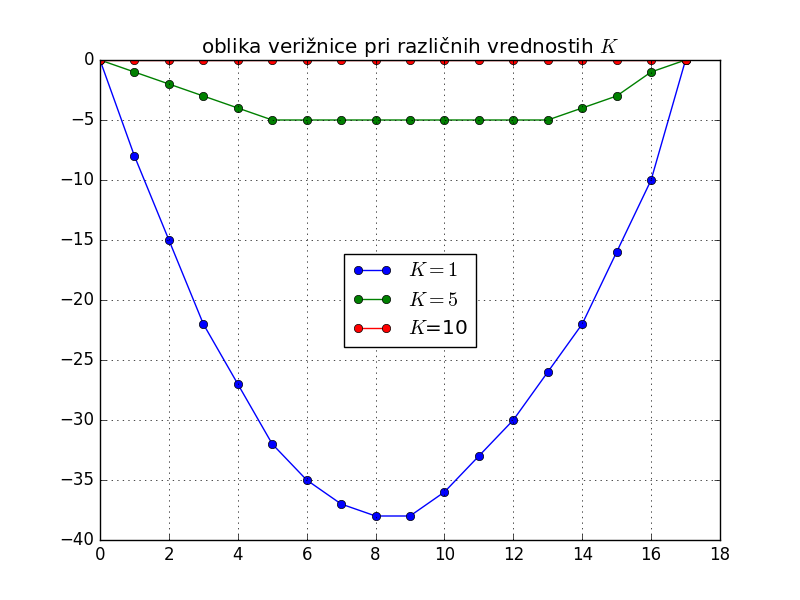
\includegraphics[scale=0.35]{slike/veriznica_temp_1.png}
%\caption{first figure}
\end{minipage}\hfill
\begin{minipage}{0.5\textwidth}
\centering
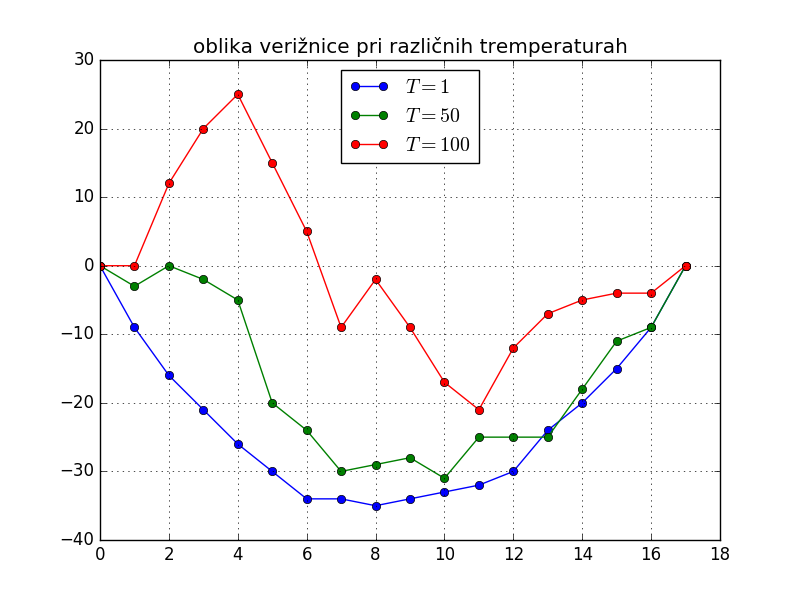
\includegraphics[scale=0.35]{slike/veriznica_k_1.png}
%\caption{second figure}
\end{minipage}

\caption{Nekaj primerov obliki verižnic. Na desnem grafu so različne rešitve pri konstantni temperaturi. Vidimo, da večji $K$, bolj poravna verižnico, saj prispevek prožnostne energije prevladuje in želi čim manjšo razdaljo med posameznimi členi. Na desnem grafu imamo verižnice pri konstantni vrednosti $K$ in pri različnih temperaturah. Opazimo, da ima verižnica bolj zapleteno obliko z večanjem temperature.}
\end{figure}


\begin{figure}[!h]
\centering
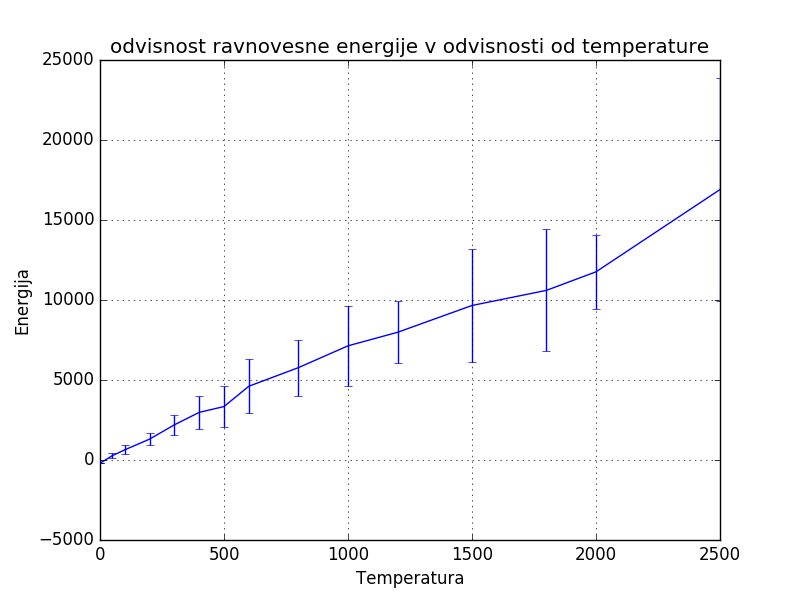
\includegraphics[scale=0.5]{slike/eviosnost_energije_od_energije_veriznica.png}
%\caption{second figure}


\caption{Odvisnost energije končnega stanja verižnice v odvisnosti od temperature. Opazimo približno linearno naraščanje energije, ki je verjetno posledica temperature, ki vzbudi sistem v višja stanja. Opazi se pa tudi večja fluktuacija energija z večjo temperaturo.}
\end{figure}

\section{Isingov model}
Isingov model opisuje feromagnetne in antiferomagnetne snovi. Z njim lahko določimo temperaturo prehoda med feromagnetnim/antiferomagnetnim stanjem in normalnim stanje. Interakcija, ki je potrebna za ta model sestoji iz dveh členov:
\begin{equation}
E=-J \sum_{<ij>} s_i s_i - H \sum_i s_i
\end{equation}
kje so $s_i$ spini atomov ter zavzemajo vrednost $\pm 1$ in vsota $<ij>$ teče po vezeh med naj bližnjimi sosedi. $H$ predstavlja zunanje magnetno polje, ki ga bomo v prvem delu zanemarili. Tokrat bomo obravnavali $2D$ model. Za iskanje termodinamskega ravnovesja postopamo podobno kot v prejšnji točki:
\begin{enumerate}
\item Izberemo začetno postavitev spinov, npr. naključno porazdeljeno z vrdostima $\pm1$,
\item izberemo naključni spin v mreži,
\item izračunamo potrebno energijo ($\Delta E$) za spremembo spina,
\item izberemo naključno številko $\rho$ na intervalu med $0$ in $1$,
\item v primeru, ko je $\rho>e^{\frac{\Delta E}{k_b T}}$ (termodinamska porazdelitev), izbranemu spinu spremenim vrednost, v nasprotnem primeru ne spremenim vrednosti spina,
\item postopek od druge točke izvajamo dokler skupna energija ne konvergira h končni točki.
\end{enumerate}
V nadaljevanju bom obravnaval le feromagnetno stanje, ker je struktura bolj zanimiva. Prav tako bomo predpostavili vrednost $J$ in $k_B$ enako $1$.
\pagebreak




\begin{figure}[!ht]
\centering
\begin{minipage}{0.5\textwidth}
\centering
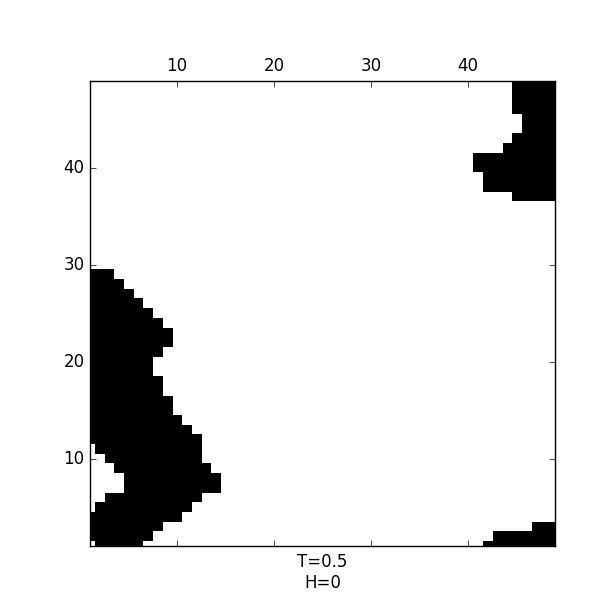
\includegraphics[scale=0.5]{slike/zunanje0T05plus.png}
%\caption{first figure}
\end{minipage}\hfill
\begin{minipage}{0.5\textwidth}
\centering
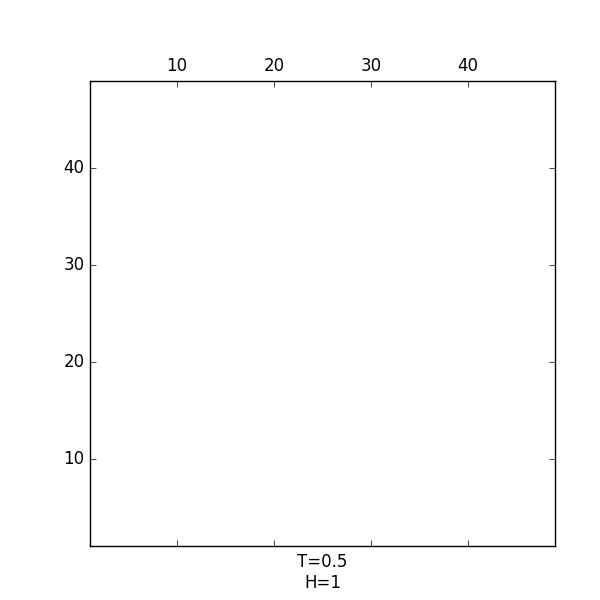
\includegraphics[scale=0.5]{slike/zunanje1T05plus.png}
%\caption{second figure}
\end{minipage}
\begin{minipage}{0.5\textwidth}
\centering
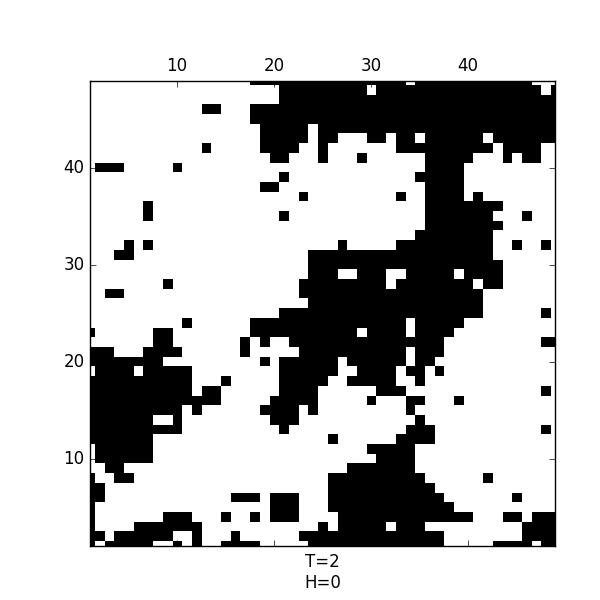
\includegraphics[scale=0.5]{slike/zunanje0T2plus.png}
%\caption{first figure}
\end{minipage}\hfill
\begin{minipage}{0.5\textwidth}
\centering
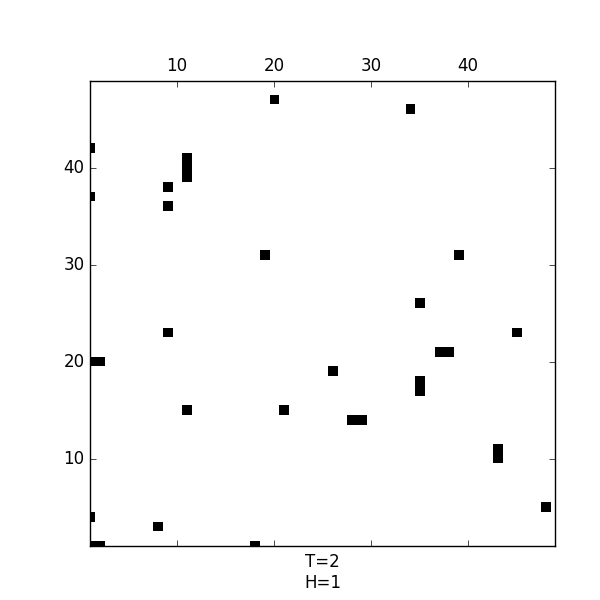
\includegraphics[scale=0.5]{slike/zunanje1T2plus.png}
%\caption{second figure}
\end{minipage}
\begin{minipage}{0.5\textwidth}
\centering
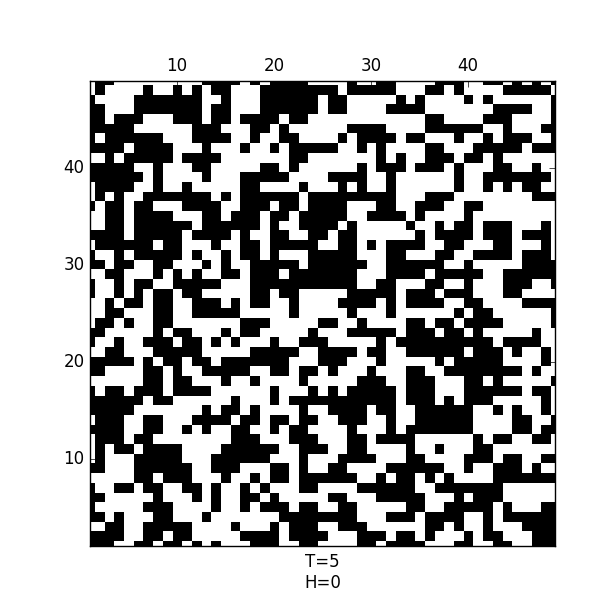
\includegraphics[scale=0.5]{slike/zunanje0T5plus.png}
%\caption{first figure}
\end{minipage}\hfill
\begin{minipage}{0.5\textwidth}
\centering
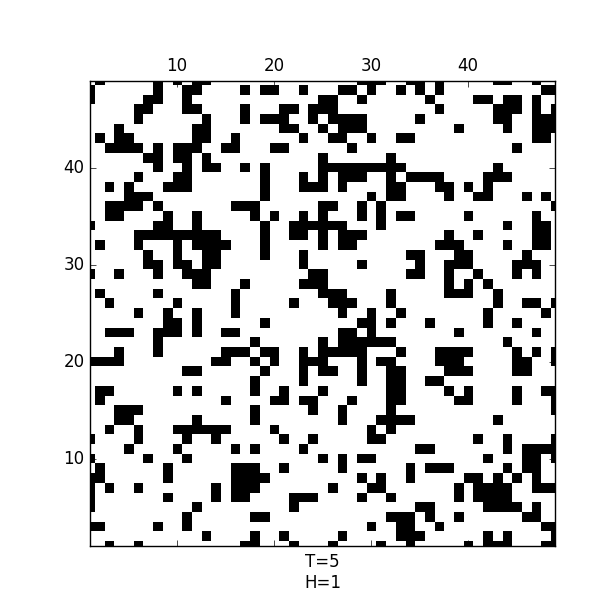
\includegraphics[scale=0.5]{slike/zunanje1T5plus.png}
%\caption{second figure}
\end{minipage}
\caption{Grafični prikaz obrnjenosti spinov za Isingov model pri različnih temperaturah in vklopljenem zunanjem polju. Bela polja predstavljajo spine $1$ ter črna polja spine $-1$. Pri nižjih temperaturah in brez zunanjega polja opazimo vzorec. Ustvarijo se domene, območja, kjer je energijsko bolj ugodno imeti spine obrnjene v enake smeri.}
\end{figure}
\pagebreak

Bolj zanimivo je ko pogledamo odvisnosti magnetizacije, susceptibilnost ter specifične toplote v odvisnosti od temperature in zunanjega magnetnega polja.
Susceptibilnost in specifično toploto izračunamo po enačbi:
\begin{equation}
\begin{aligned}
x\chi =& \frac{\braket{S^2} -\braket{S}^2}{k_B T} \\
c =& \frac{\braket{E^2} -\braket{E}^2}{k_B T^2}
\end{aligned}
\end{equation}


Pričakovani vrednosti povprečne energije in spina izračunamo: $S=\frac{1}{N} \sum_1^N s_i$. V primeru ko ni zunanjega magnetnega polja, se lahko izračuna kritično temperaturo $T_c$, pri kateri pride do faznega prehoda. Ta vrednost je: $T_c \approx 2.2691 \frac{J}{k_B}$.


\begin{figure}[h]
\centering
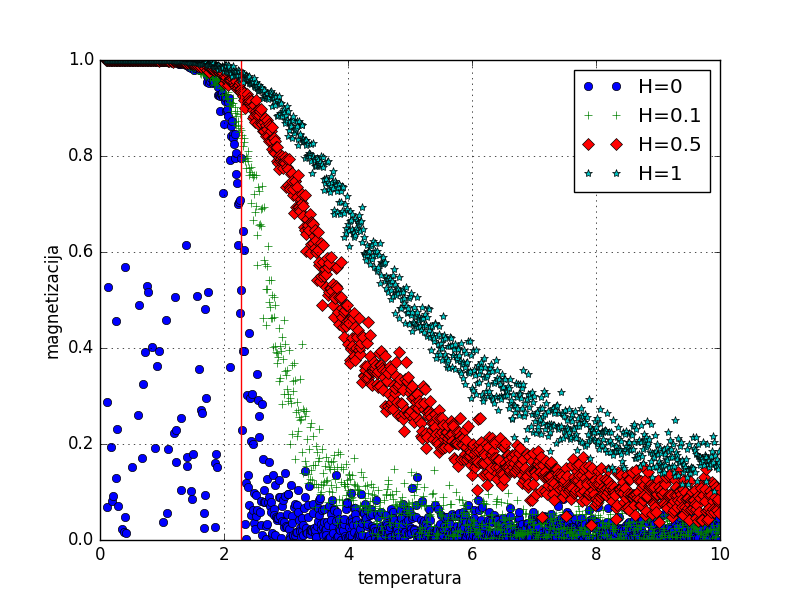
\includegraphics[scale=0.7]{slike/magneizacija_tudi_zunanje2.png}
\caption{Magnetizacija v odvisnosti od temperature. Opazimo fazni prehod pri kritični temperaturi (rdeča navpična črta), ko je zunanje polje enako $0$. Pri vklopu zunanjega polja je prehod med fazama bolj položen (manj izrazit) in pri višji temperaturi.}
\end{figure}


\begin{figure}
\centering
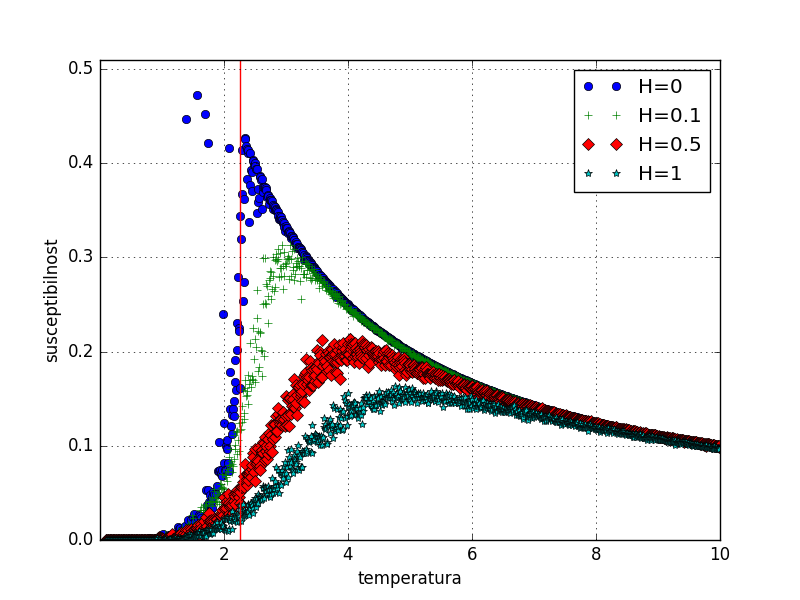
\includegraphics[scale=0.7]{slike/susceptibilnost1.png}
\caption{Odvisnost susceptibilnost od temperature. Opazimo da se maksimum susceptibilnosti z zunanjem poljem premika v desno, kar potrjuje hipotezo, da z večjim zunanjim poljem temperatura faznega prehoda večja.}
\end{figure}


\begin{figure}
\centering
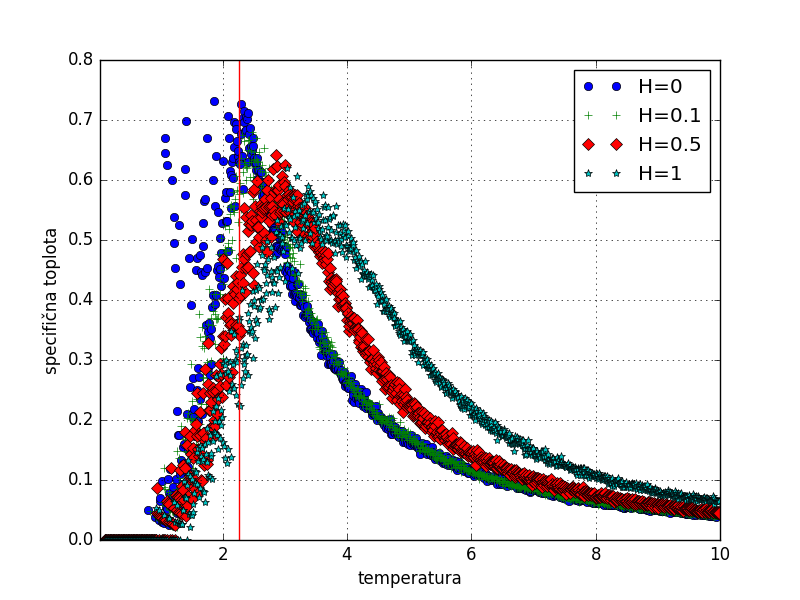
\includegraphics[scale=0.7]{slike/specificna1.png}
\caption{Graf specifične toplote v odvisnosti od temperature. Opazimo, da imajo ti grafi najbolj izrazit vrh in lahko iz njih najlažje določimo temperaturo faznega prehoda.}
\end{figure}


























\end{document}
